% !TeX program = lualatex
% Author         : Pedro Ferreira (up201806093@up.pt)
% Version        : 1.0
% Created on     : 12.08.2022
% Last Edited on : 14.08.2022
% Adapted from HSRM theme by Benjamin Weiss
% Copyright      : Copyright (c) 2013-2014 by Benjamin Weiss. All rights reserved.
% License        : This file may be distributed and/or modified under the
%                  GNU Public License.
% Description    : HSRM beamer theme demonstration. Also includes a short 
%                  Tutorial regarding the beamer class.



%%%%%%%%%%%%%%%%%%%%%%%%%%%%%%%%%%%%%%%%%%%%%%%%%%%%%%%%%%%%%%%%%%%%%%%%%%%
%                    !!! Compile with LuaLaTex !!!
%%%%%%%%%%%%%%%%%%%%%%%%%%%%%%%%%%%%%%%%%%%%%%%%%%%%%%%%%%%%%%%%%%%%%%%%%%%

\documentclass[compress,aspectratio=169]{beamer}
%--------------------------------------------------------------------------
% Common packages
%--------------------------------------------------------------------------
\usepackage[french]{babel}
\hypersetup{
pdftitle={Présentation de pré-étude},
pdfsubject={Pré-étude},
pdfauthor={Ali Zoubir},
pdfkeywords={Latex,Beamer}}

\usepackage{graphicx}
\usepackage{multicol}

% Advanced table functions
\usepackage{tabularx,ragged2e}
\usepackage{booktabs}
% Listings extension
\usepackage{listings}
\lstset{ %
language=[LaTeX]TeX,
basicstyle=\normalsize\ttfamily,
keywordstyle=,
numbers=left,
numberstyle=\tiny\ttfamily,
stepnumber=1,
showspaces=false,
showstringspaces=false,
showtabs=false,
breaklines=true,
frame=tb,
framerule=0.5pt,
tabsize=4,
framexleftmargin=0.5em,
framexrightmargin=0.5em,
xleftmargin=0.5em,
xrightmargin=0.5em
}

%--------------------------------------------------------------------------
% Load theme
%--------------------------------------------------------------------------
\usepackage{sleektheme/beamerthemesleek}
\usetheme[]{sleek}

\usepackage{sleektheme/dtklogos} % must be loaded after theme
\usepackage{tikz}
\usetikzlibrary{mindmap,backgrounds}

%--------------------------------------------------------------------------
% General presentation settings
%--------------------------------------------------------------------------
\title{Présentation pré-étude}
\subtitle{Localisation sous-marine 2221 \\ {\small Système de logging pour algorithme de localisation sous-marine}}
\date{Dérnière MAJ: \today}
\author{Ali Zoubir}
\institute{ETML-ES\\ {\Medium Génie électrique}}

%--------------------------------------------------------------------------
% Notes settings
%--------------------------------------------------------------------------
\setbeameroption{show notes}

\begin{document}
%--------------------------------------------------------------------------
% Titlepage
%--------------------------------------------------------------------------

\maketitle

%\begin{frame}[plain]
%	\titlepage
%\end{frame}

%--------------------------------------------------------------------------
% Table of contents
%--------------------------------------------------------------------------
\section*{Structure}
\begin{frame}{Structure}
	% hideallsubsections is recommended for longer presentations
	\tableofcontents[hideallsubsections]
\end{frame}

%--------------------------------------------------------------------------
% Content
%--------------------------------------------------------------------------
\section{Introduction}

\begin{frame}{Présentation du projet}
	L'objectif de ce projet, et de stocker des données de mesures du déplacement d'un module sous-marin
	par une centrale inertielle, dans le but de le localiser.\vspace{-4pt}
	\begin{figure}
		\centering
		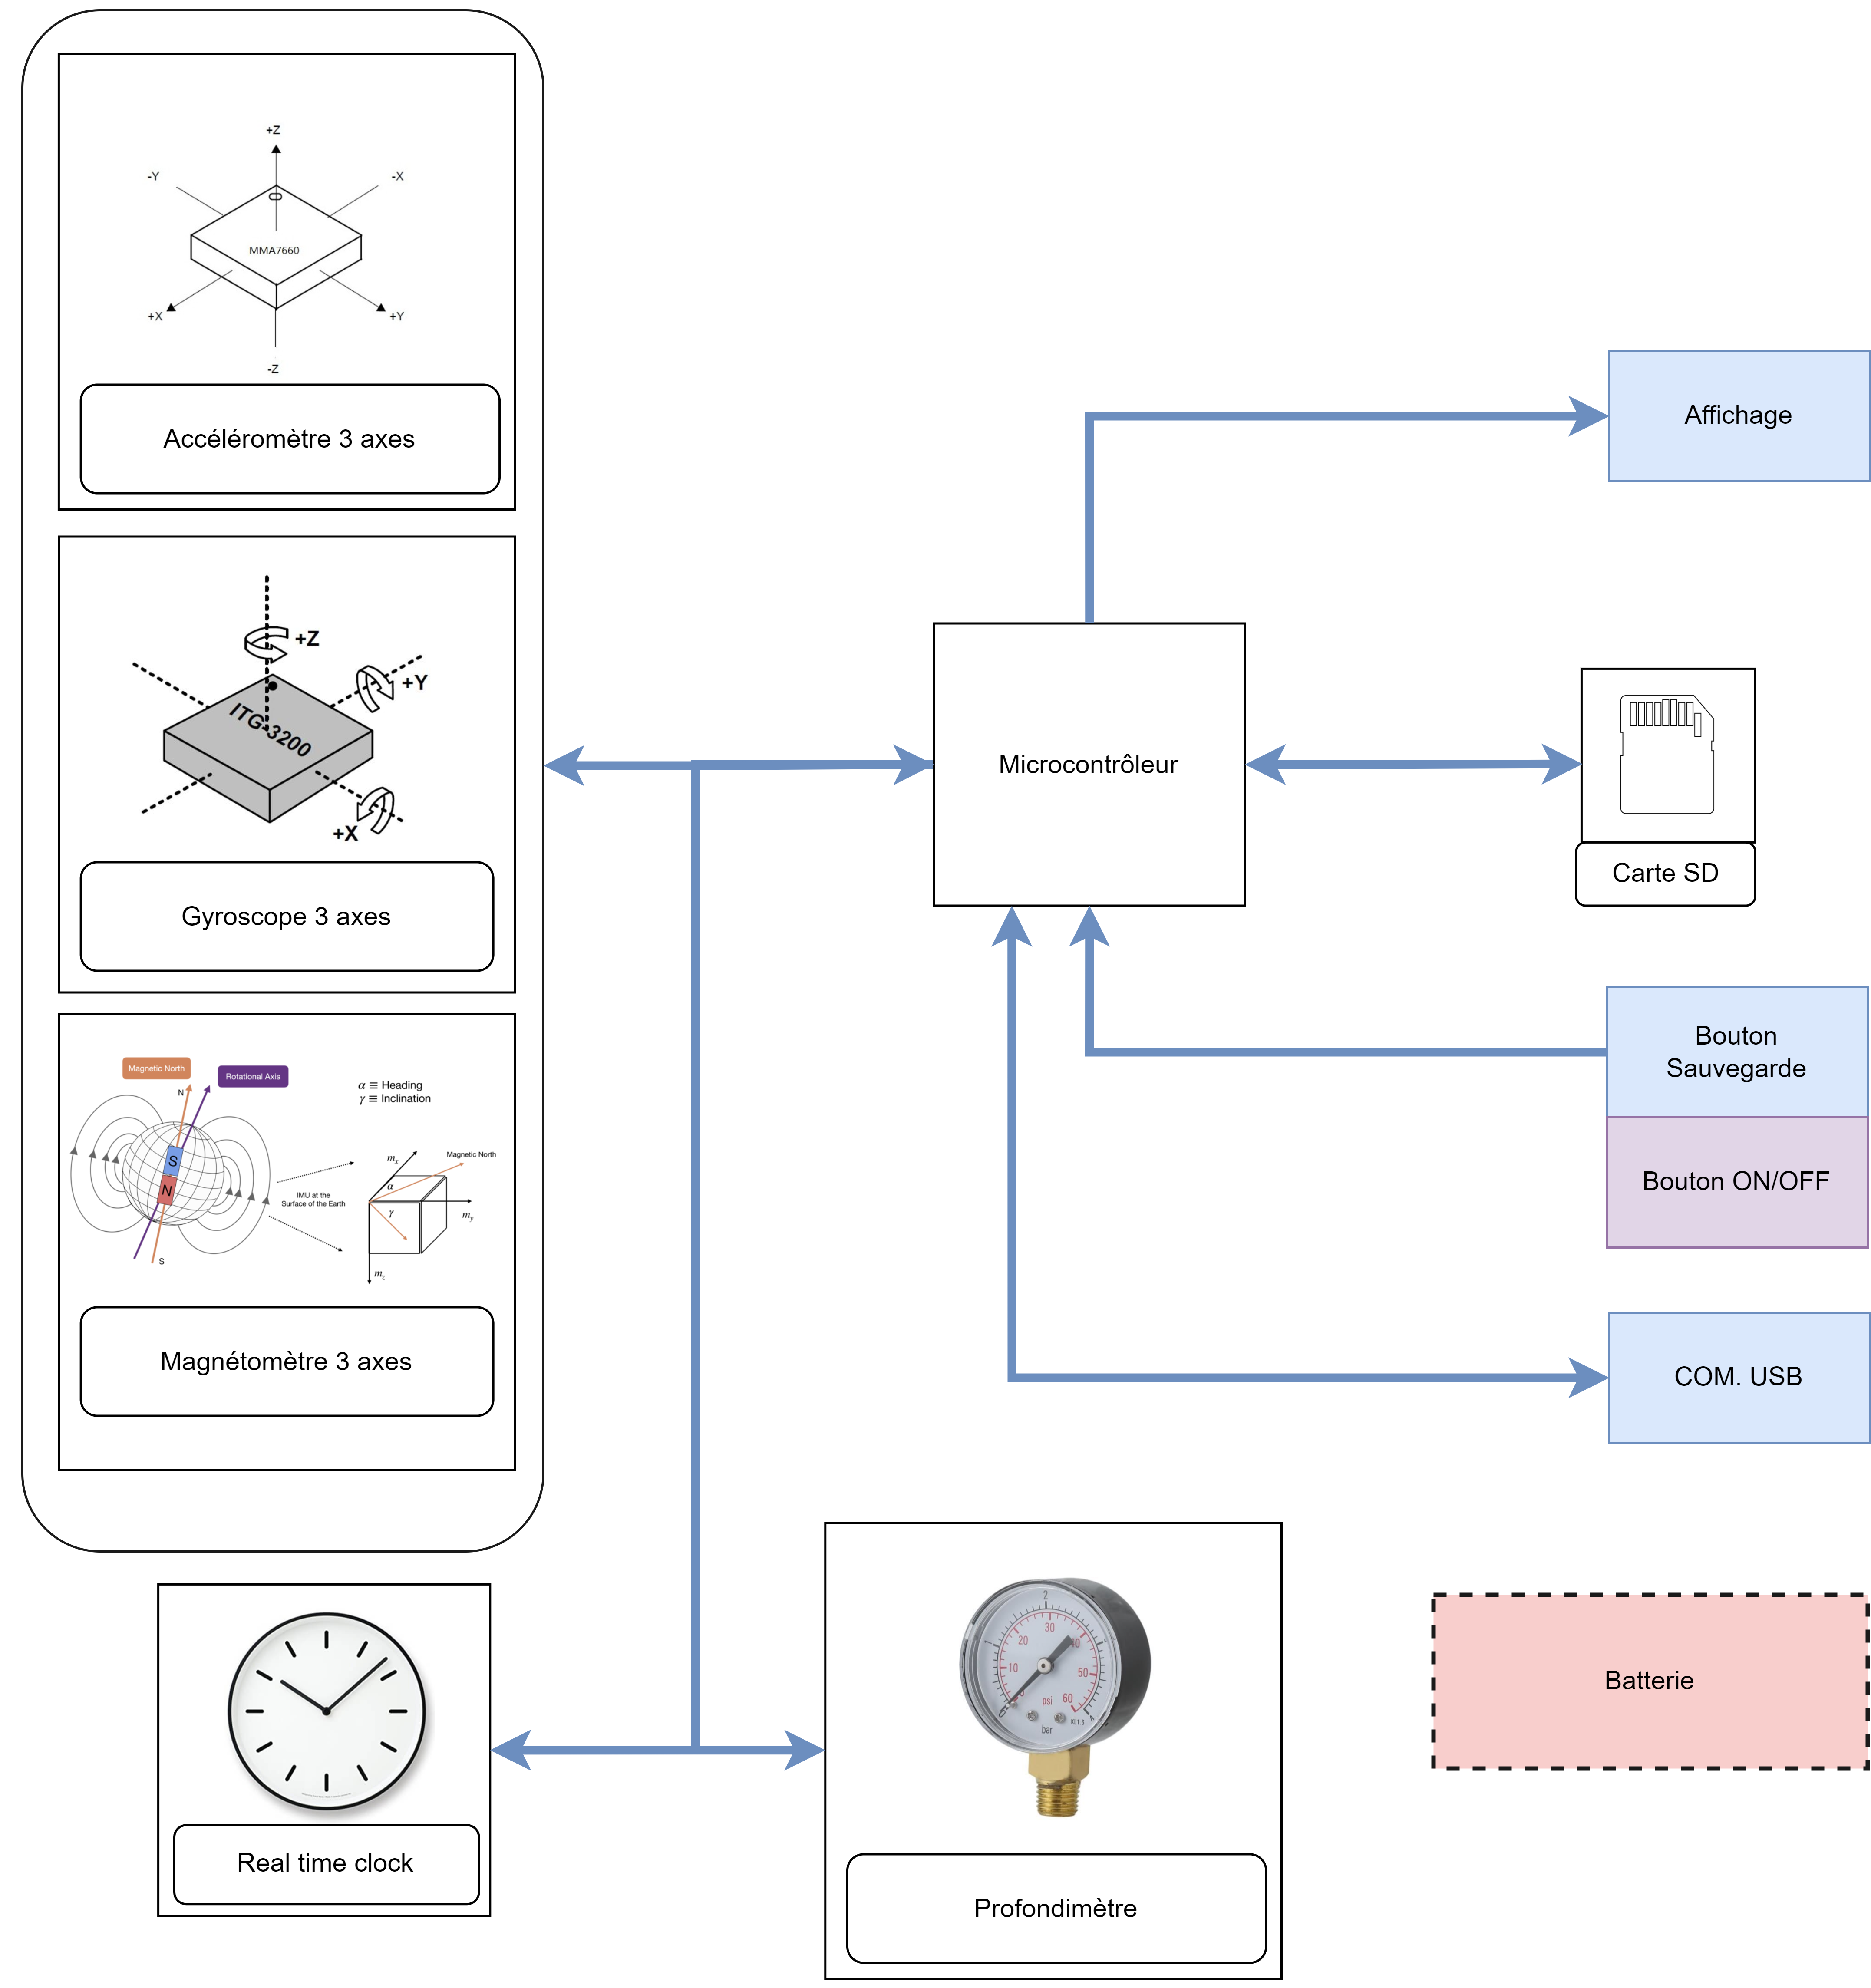
\includegraphics[width=0.4\linewidth]{Images/pre-etude.drawio}
	\end{figure}
	

\end{frame}

\begin{frame}{Caractéristiques}
	\begin{alertblock}{Principales}
		Sensing sur 9 axes. \\
		Sauvegarde d’un set de donnée chaque 100ms.\\
		2 heure de logging dans une carte SD. \\
		Possibilité de sauvegarder la localisation de points d’intérêts. \\
		Profondeur d’utilisation maximum, de 60m. \\ 
		Batterie, autonomie minimum de 2 heures \\
		Charge de la batterie par connecteur USB.
	\end{alertblock}
	\begin{exampleblock}{Secondaires}
		Lecture des données par connecteur USB (Interfaçage électronique, software
		optionnel dans cette version). \\
		Interface LED ou petit écran.
	\end{exampleblock}
\end{frame}

\section{Déroulement}

\begin{frame}[containsverbatim]{Tâches à réaliser}
	Développement et intégration d’un PCB avec capteurs et logging sur carte SD dans une lampe de plongée étanche.
	\begin{itemize}
		\item[•] Développement schématique 
		\\ \quad Fonctionnement MCU. 
		\\ \quad Périphériques de mesures et de sauvegarde / Bus de communication. 
		\\ \quad Gestion batterie 
		\item[•]	Routage pour intégration dans boitier de lampe de plongée 200x45mm.
		\item[•]	Programmation mesure et sauvegarde chaque 100ms.
		\\	\quad Configuration MCU.
		\\	\quad Configuration des périphériques de mesure pour 9-DOF.
		\\	\quad Configuration des périphériques de sauvegarde (Carte SD).
		\\	\quad Configuration et communication avec l'interface.
		\\	\quad Communication et traitement des données mesurées.
	\end{itemize}
\end{frame}

\begin{frame}
	\vspace{+3mm}
	\begin{block}{Carte SD}
		Stockage des données de mesures chaque 100ms, coeur du projet.
	\end{block}

	\begin{block}{Profondimètre}
		Permet de déduire la profondeur, afin de corroborer les autres mesures des capteurs.
	\end{block}

	\begin{block}{Affichage}
		Affichage LED ou écran, pour affichage  (ex. Profondeur, état batterie. . .)
	\end{block}
	
	\begin{block}{Bouton interface}
		 Bouton ON/OFF et mise en valeur d’un set de mesure.
	\end{block}
	
	\begin{block}{COM. USB}
		Permet de charger les batteries, enregistrer les données et de calibrer la RTC.
	\end{block}
\end{frame}
 

\section{Dimensionnements}
\begin{frame}[containsverbatim]{Schéma bloc détaillé}
	\begin{figure}[h]
		\centering
		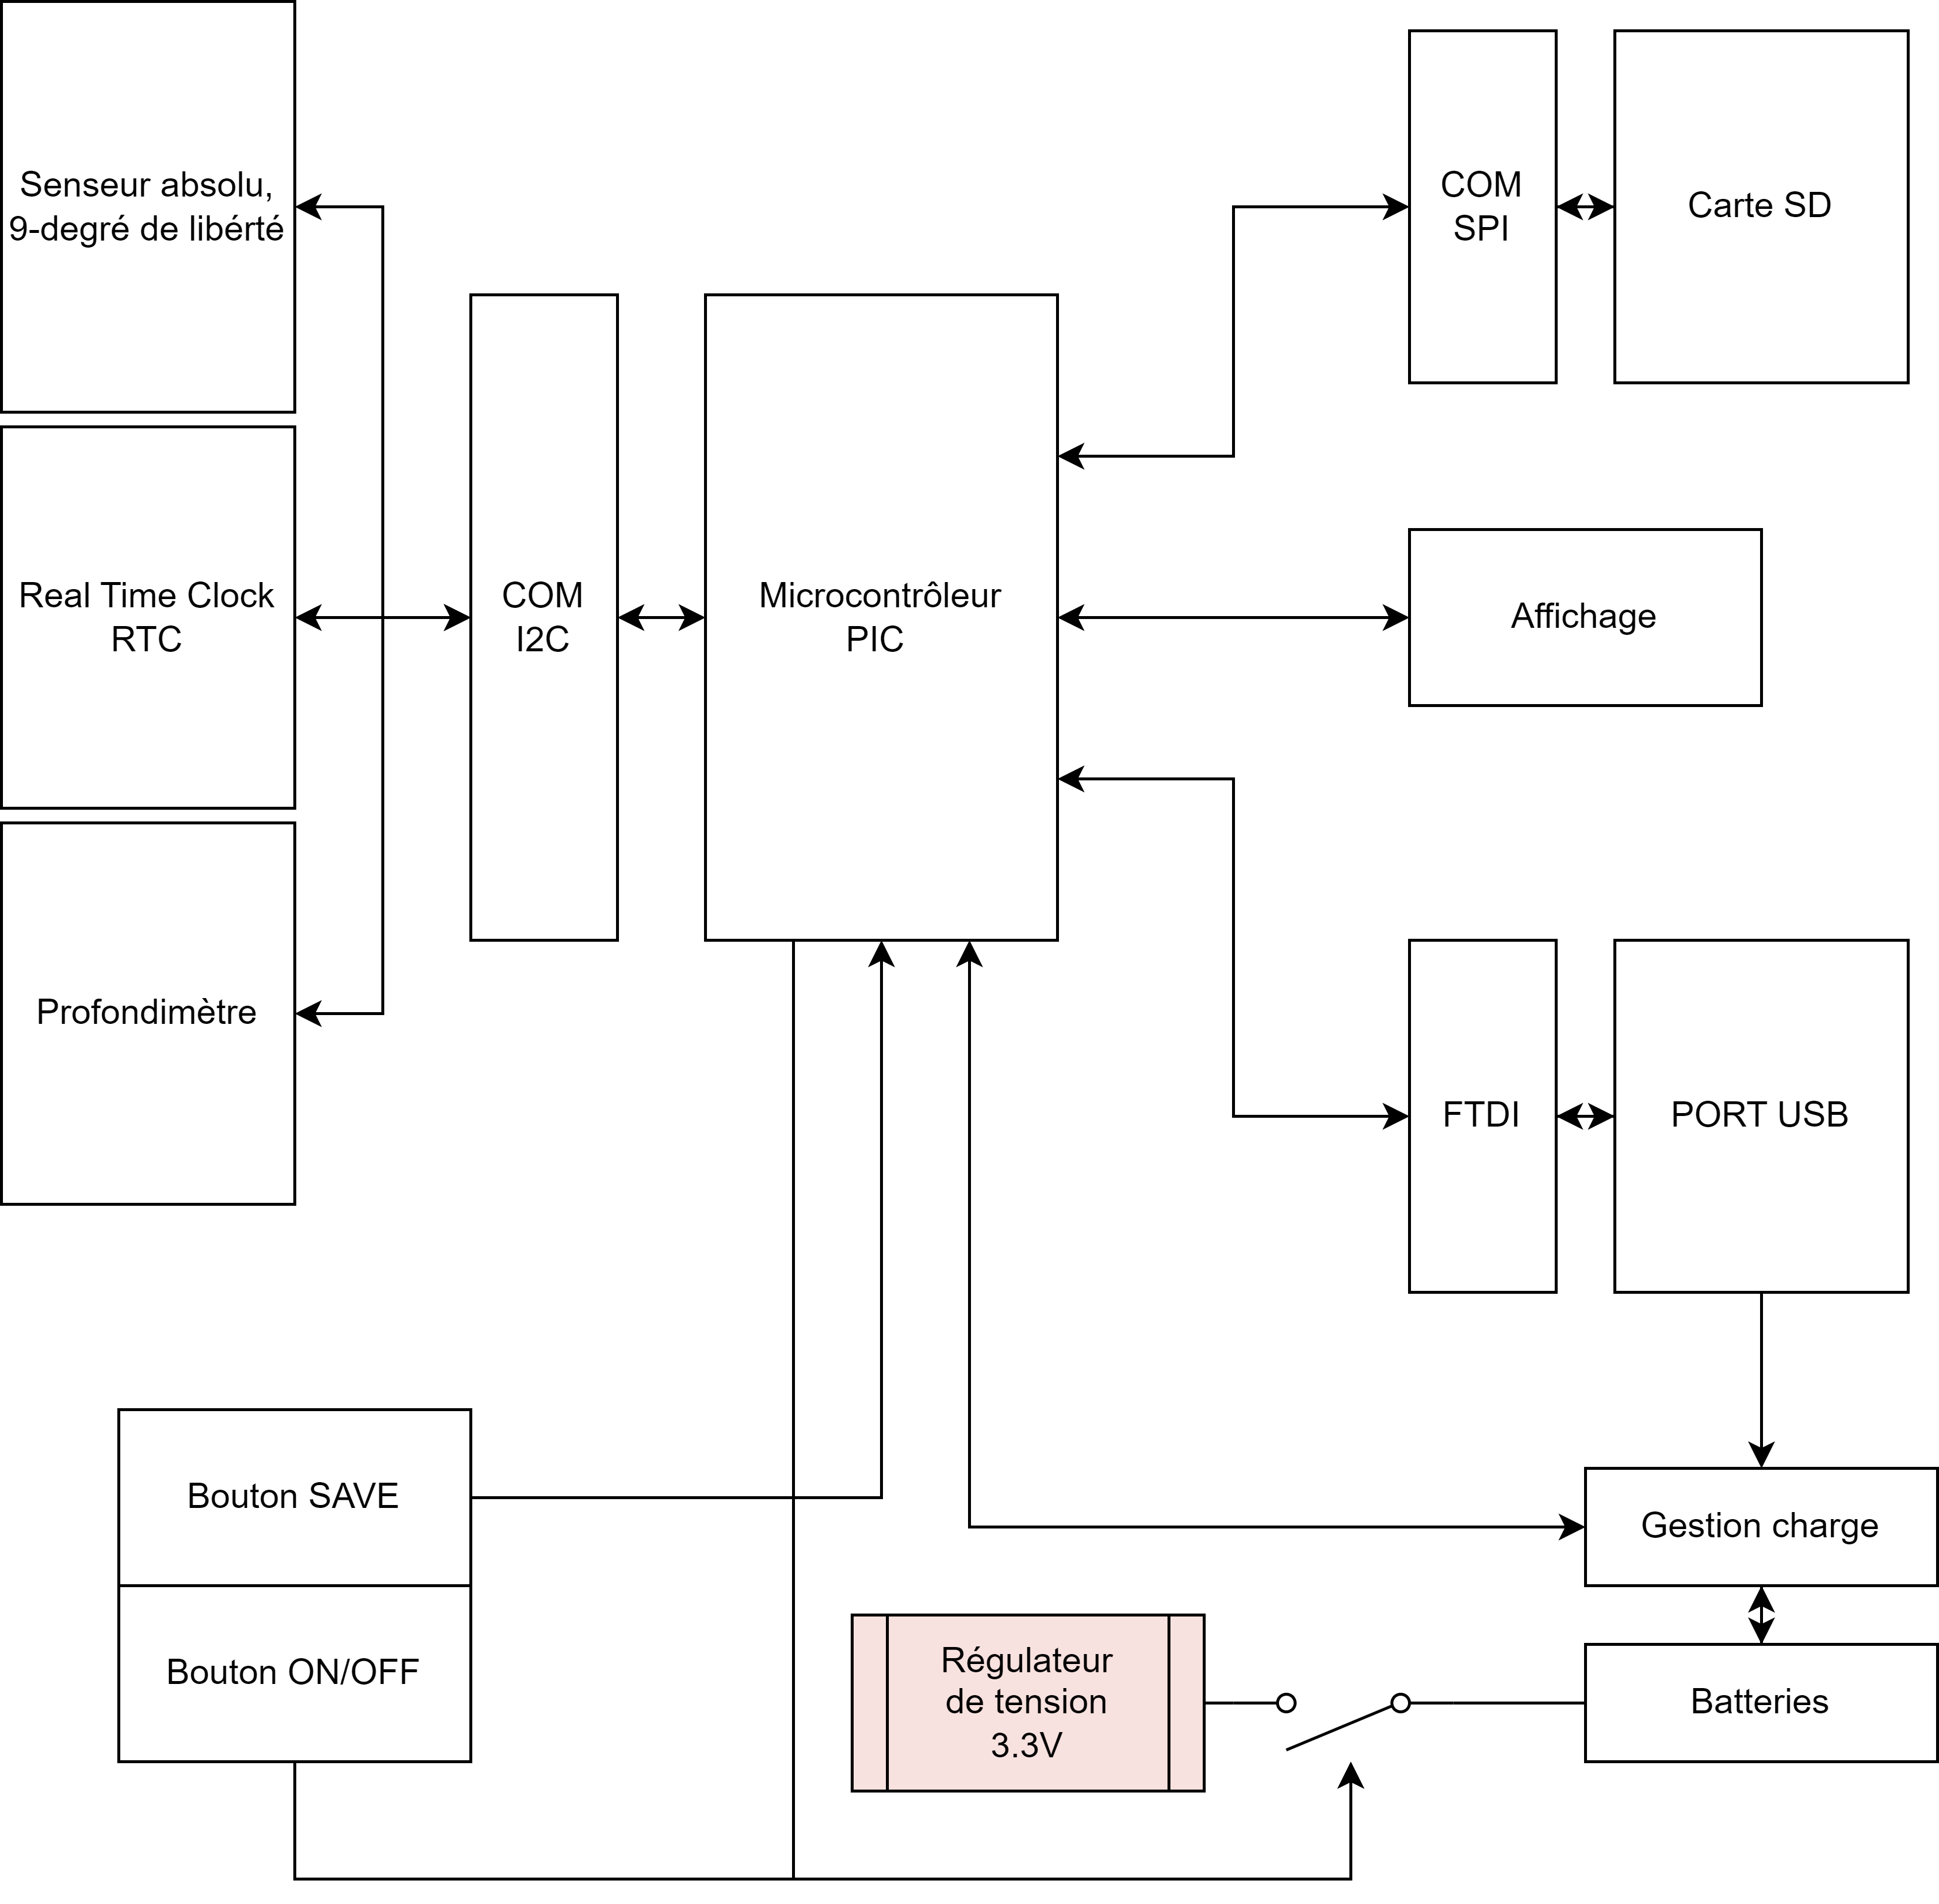
\includegraphics[width=0.5\linewidth]{Images/Schema-bloc-LocalisationSousMarin}
	\end{figure}
\end{frame}

\begin{frame}[containsverbatim]{Schéma bloc - connexions}
	\begin{figure}[h]
		\centering
		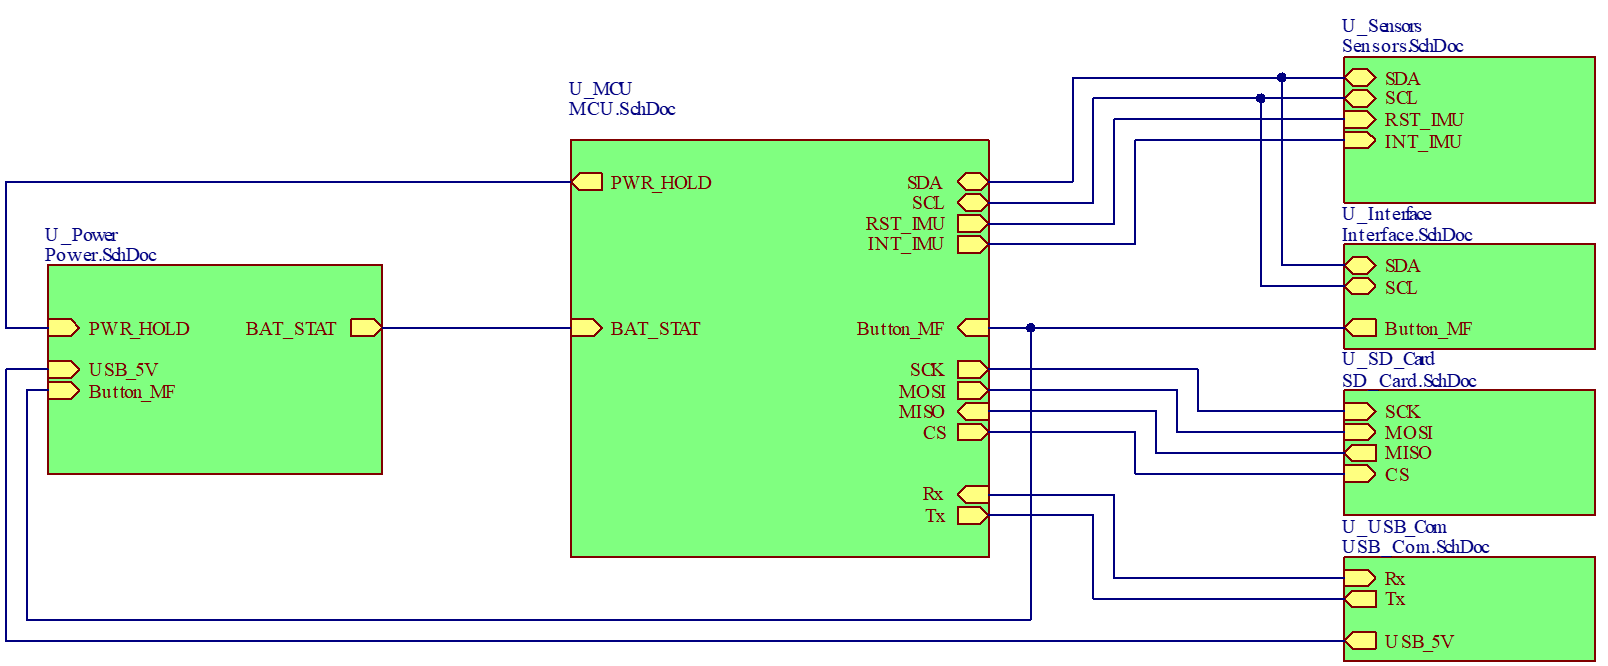
\includegraphics[width=1\linewidth]{Images/Altium-blocks}
	\end{figure}
\end{frame}

\begin{frame}[containsverbatim]{Centrale inertielle}
	\begin{figure}
		\centering
		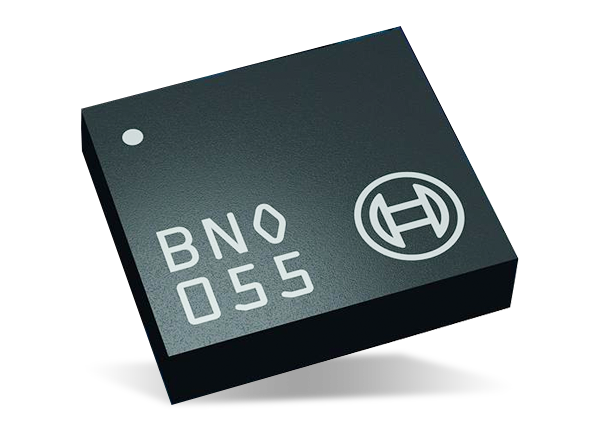
\includegraphics[width=0.3\linewidth]{Images/BNO055-Illustration}
	\end{figure}
	\begin{tabular}{l l l l}
		Résolution gyroscope & : & 16 & [bits] \\
		Résolution accéléromètre & : & 14 & [bits] \\
		Résolution magnétomètre & : & $\sim$0.3 & [$\mu$T] \\
		$I_{DD}$ & : & 12.3 & [mA] \\
		Dérive de température & : & $\pm$ 0.03 & [\%/K] \\ 
		Dérive accéléromètre & : & 0.2 & [\%/V] \\
		Dérive gyroscope & : & <0.4 & [\%/V]
	\end{tabular} \\
\end{frame}

\begin{frame}[containsverbatim]{Carte SD}
	\begin{figure}
		\centering
		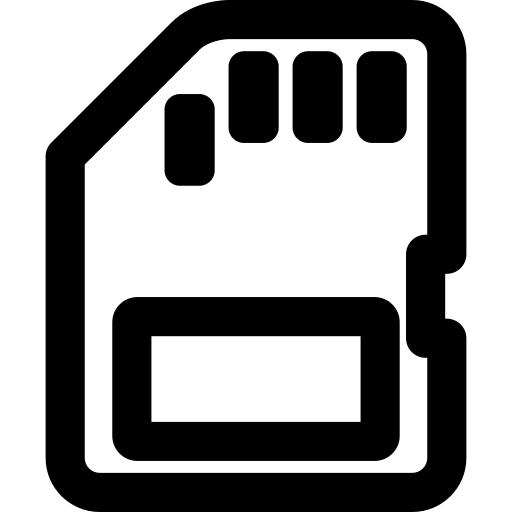
\includegraphics[width=0.1\linewidth]{Images/SDcard}
	\end{figure}
	\begin{tabular}{l l ll|l}
		$ T_{rec} $ & = &  $7200'000$ & $[ms]$ & Temps a enregistrer \\
		$ T_{ech}$ & = & $100$  & $[ms]$ & Temps d'un échantillon \\
		$ S_{mes} $ & = & $43$ & $[bytes]$ & Taille de toutes les données de mesures  \\
		$ S_{timestamp} $ & = & $\sim$23 & $[bytes]$ & Taille de l'information de temporalité  \\
		$ S_{flag} $ & = & $ 1 $ & $[bytes]$ & Taille de l'indication d'importance 
	\end{tabular}
    \begin{equation} \label{equ:NbMes}
		Nb_{mesures} = \frac{T_{rec}}{T_{ech}}
	\end{equation} 
	\begin{equation} \label{equ:TailleMin}
		Taille_{min} = Nb_{mesures} * (S_{mes}+S_{timestamp}+S_{flag}) 
	\end{equation}
	
	\textbf{72'000} Mesures et \textbf{5MB} de taille mémoire
\end{frame}

\begin{frame}[containsverbatim]{Technologie des batteries}
	\par
	\raisebox{-.5\height}{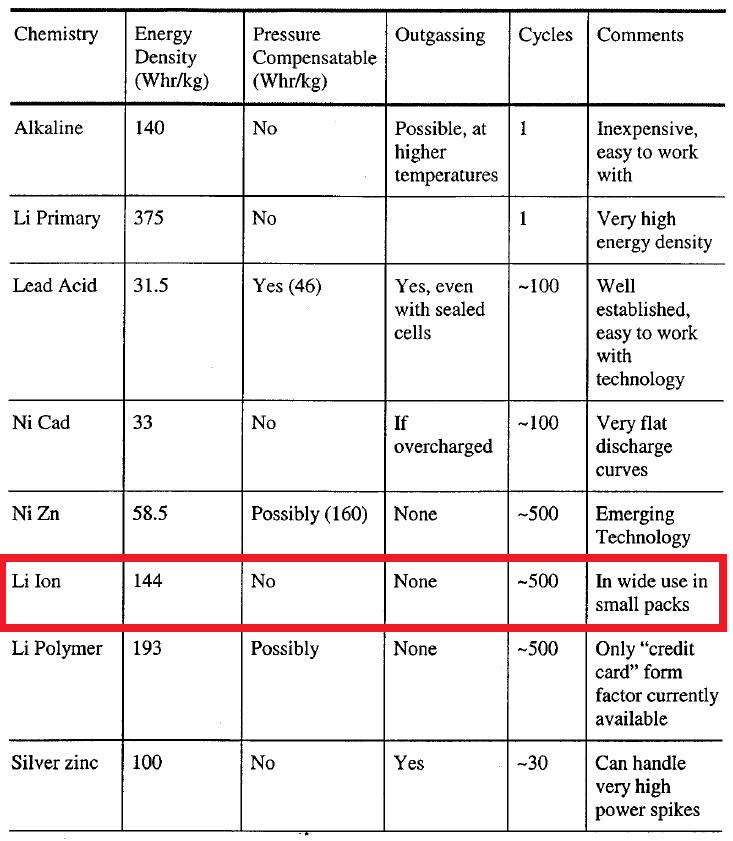
\includegraphics[width=5cm]{Images/PowerSystemsComparison}}%
	\begin{tabular}{c|c}
		Avantages &  Inconvénient\\
		\hline
		Haute densité d'énergie & Risque d'éclatement \\
		Poids léger & Risque d'enflammement (eau) \\ 
		Haute durée de vie & Sensible a la température \\
		Charge rapide & Décharge complète altérante \\
	\end{tabular}
	\par
\end{frame}

\begin{frame}[containsverbatim]{Estimation des coûts}
	\begin{center}
		\begin{tabular}{l|l}
			Composant & Estimation \\
			\hline
			Profondimètre & 70.- \\
			Centrale inertielle & 35.- \\
			RTC & 5.- \\
			Microcontrôleur & 15.- \\
			Carte SD & 20.- \\
			Affichage OLED & 45.- \\
			FTDI & 4.- \\
			Batterie LI-ION & 20.- \\
			IC chargeur & 4.- \\
			Régulateur 3.3V & 10.- \\
			PCB & 100.- \\
			\hline
			\hline
			\vspace{+5pt}Total & 328.-
		\end{tabular} 
	\end{center}
\end{frame}

\section{Conclusion}

\begin{frame}[containsverbatim]{Conclusion et perspectives}
	J’ai pu lors de cette pré-étude, établir le fonctionnement global du système,
	choisir certaines technologies et composants importants, ainsi que
	pu procéder a certains dimensionnements utiles quant au futur développement.
	
	
	Par la suite, je vais affiner les différents éléments abordés lors de la
	pré-étude, effectuer le développement plus détaillé de chacun des blocs et
	réaliser la schématique du projet.
	
	
	Lors de la pré-étude, je n’ai pas eu accès au boîtier mécanique du projet,
	ce qui a restreint mon champs d’action lors de certains dimensionnement,
	tandis que pendant l’étude j’aurais accès a celui-ci, ce qui risque d’impacter/
	modifier certains aspect fixés lors des section antérieures.
\end{frame}

\begin{frame}{References}
	\begin{thebibliography}{10}
    
    \beamertemplatearticlebibitems
    \bibitem{BAT2021}
    Singh H., Yates S. F.
    \newblock \doublequoted{Review of issues related to the design of battery systems and energy transfer (charging) techniques for autonomous underwater vehicles (AUVs) operating within an autonomous ocean sampling network (AOSN).}
    \newblock 2021
    
	\beamertemplatearticlebibitems
	\bibitem{FUSION021}
	Shaukat N., Ali A., Javed I., Moinuddin M., Otero P.
	\newblock \doublequoted{Multi-Sensor Fusion for Underwater Vehicle Localization by Augmentation of RBF Neural Network and Error-State Kalman Filter}
	\newblock 2021

	\beamertemplatearticlebibitems
	\bibitem{BREV}
	Zaki, Ahmed S., Straw, Timothy B., Obara, Michael J., Child, Peter A. 
	\newblock \doublequoted{Brevet : High accuracy heading sensor for an underwater towed array}
	\newblock 2014
	
  \end{thebibliography}
\end{frame}

\end{document}






